\documentclass{article}

\usepackage{todonotes}
\usepackage[colorlinks=true]{hyperref}
\usepackage[framed,numbered,autolinebreaks]{mcode}
\usepackage{fullpage}
\usepackage{url,textcomp}
\setlength{\parindent}{0pt}
\setlength{\parskip}{18pt}
\title{MATLAB Introduction}
\author{Rob Campbell \& Maxime Rio}
\date{}
% //////////////////////////////////////////////////

\renewcommand{\familydefault}{\sfdefault}
\usepackage{helvet}
\usepackage[compact]{titlesec}
\titlespacing\subsection{0pt}{12pt plus 4pt minus 2pt}{0pt plus 0pt minus 5pt}

\begin{document}

\maketitle


\section*{Introduction}

MATLAB is a fairly simple programming language designed to make analysis of data easy.
It is commonly used in academic research, industry, and finance.
It is used across scientific disciplines, from biologists to engineers.
During this course, you will use MATLAB to analyse existing 2-photon imaging data from mice, acquire new action potential data with electrodes, and analyse these data.
Today you will learn the basics of MATLAB.

MATLAB stores data in \textbf{variables} and these variables are manipulated by \textbf{functions}.
There are simple functions for performing tasks such as multiplication and division.
There are also more complex functions for doing things such as calculating averages, fitting lines, and doing statistical tests.
Today you will learn the basic functions in MATLAB as well as how to chain these together using \textbf{loops} and \textbf{logic statements} to automate sequences of operations.
This is the basis of programming.

As you proceed you will doubtless get stuck.
For help you should use the MATLAB documentation that is built-in, Google, and ask for assistance.


\section{Starting MATLAB}

\todo[inline]{Start MATLAB from the Windows start menu.}
\todo[inline]{Add section on navigating the command line window, opening an m-file, and the system path.}
\todo[inline]{Describe the ribbon.}


\section{Working at the command line}

We will begin by treating MATLAB as a graphical calculator.
We will start off at the \textbf{command line}, where you see the \verb|>>| symbol.
You type commands in the space after the \verb|>>| symbol.

Take a deep breath and type a number into the command line, e.g. \\
\verb|>>| \mcode{1} \\
then press return. \\
See how it echoes the number back to you? Now type: \\
\verb|>>| \mcode{1;} \\
Note the presence of the \mcode{;} symbol.
See how it no longer echoes the number back to you?
The \mcode{;} suppresses the echo.
You will use this feature a lot so keep it in mind.

Number are not limited to positive integers.
You can also enter real numbers, for example \\
\verb|>> 0.012| \\
or with a scientific notation \\
\verb|>> 1.2e-2| \\
and negative values, using a \mcode{-} (minus) sign:\\
\verb|>> -3.5| \\

Now let's look at basic arithmetic operators.
Type the following into the command line (note we leave off the semicolon so you can see the output):
\begin{lstlisting}
4 + 10
4 - 10
4 * 10
4 / 10
4^3
\end{lstlisting}
What does the last line \mcode{4^3} do?

Of course you can use several operators in the same line, but be careful with their priority.
You can force the order of the operations using parentheses.
Compare the results from the following lines:
\begin{lstlisting}
4 + 2 * 3 - 1
(4 + 2) * 3 - 1
(4 + 2) * (3 - 1)
\end{lstlisting}

To conclude this first part, enter the following into the command line: \\
\verb|>>| \mcode{\%This is a comment.} \\
After pressing return, nothing should have happened.
Indeed, any lines starting with the \mcode{\%} symbol are \verb|comments| and aren't executed by MATLAB.
We will use these comments to provide additional information to you.


\section{Manipulating simple variables}

A variable is a mechanism to keep track of a value with a name.
Variables are assigned with the \mcode{=} (equals) operator.
The name of a variable is on the left of \mcode{=} and the value on the right, e.g.\\
\verb|>> myvariable = 12|

Type the following into the command line.
Remember, you don't need to type the comments, those are just to explain what is going on.
\begin{lstlisting}
t = 1      % assign the number 1 to a variable called t
r = 10.5;  % create another variable (note lack of echoing)
a = r      % assigning one variable to another
a          % display the value of the variable
\end{lstlisting}

If you assign several times values to the same variable, values are replaced in turns.
\begin{lstlisting}
t = 2  % previous value replaced by 2
t = 3  % value 2 replaced by 3
\end{lstlisting}

You can use variables in place of values for arithmetic operations.
Type the following in the command line:
\begin{lstlisting}
t = 2;
T = t + 10  % addition
T = t - 10  % subtraction
T = t * 2   % multiplication
T = t / 10  % division
T = t^3     % raising to the third power
\end{lstlisting}

By the way, what is the final value of \mcode{T}? and \mcode{t}?
Be careful, variables names are case sensitive, so \mcode{T} and \mcode{t} are different variables!
\todo{talk about fine names for variables?}

If you want to know about the currently used variables, have a look to the \textbf{workspace} panel.
There you will see names and values of your variables.

So far, we have only been manipulating variables containing numbers, but other types of data can be used.
For example, a sequence of characters, also known as \textbf{string}, is defined by enclosing any text with single quotes.
Try the following in the command line:
\begin{lstlisting}
'my first string!'         % create a string and echo it
b = 'and the second one';  % assign a string to a variable, without echoing
\end{lstlisting}
This type of variable is useful to print custom messaged, as we will see later on.
Keep that in a corner of your head.

Sometimes, one may want to delete a variable, because it is not used anymore and use a lot of memory.
To do so, you will use the \mcode{clear} command.
Type the following in the command line and check how the \textbf{workspace} panel changes:
\begin{lstlisting}
clear    % remove all variables
a = 3    % new variable
b = 4    % new variable
clear a  % remove one variable
c = a    % assign a variable to another one and... surprise!
\end{lstlisting}
What happened at last line? Keep in mind that a variable need to exist in order to be used.


\section{Using MATLAB functions}

So far, you were limited to basic arithmetic.
What if you want to do more advanced math? or control a little bit the interface?
For these cases, MATLAB provides a huge number of functions to do all sort of operations.

To use a function, you need to type its name.
In the command line, try typing \mcode{clc} and see what happens.

If you want to now more about this function, you can use \mcode{help} command as follows: \\
\verb|>> help clc| \\
You can also use \mcode{doc} command to get an extended help, typing \mcode{doc clc}.

A function can have inputs and outputs.
Inputs are enclosed in parenthesis, after the function name, and separated by commas.
You get back the output(s) using variable assignment.

Give a try with the \mcode{cos} function (cosine of an angle), typing the following:
\begin{lstlisting}
clear         % remove all previously defined variables
cos(3.14)     % cosine of Pi
x = 3.14;     % create a new variable (no echoing)
cos(x)        % cosine of the value of x
y = cos(x);   % assign the result to a variable (no echoing)
\end{lstlisting}

What about a function that takes several inputs?
Have a look to \mcode{rem} function, using \mcode{help} or \mcode{doc} command.
Use this function to compute the remainder after division of 823 by 11.

Some function can have optional inputs.
A good example is the \mcode{round} function.
Check its documentation using \mcode{help} to understand the difference between the following lines:
\begin{lstlisting}
clear  % remove all variables
x = 4568.12;
r1 = round(x);
r2 = round(x, 0);
r3 = round(x, -2);
\end{lstlisting}
What are the values in variables \mcode{r1}, \mcode{r2} and \mcode{r3} at the end?

Congratulations, you've now learned the basics of entering information into the command-line.
\todo{add a example with mod}

\section{Writing your own functions}

A MATLAB \textbf{function} is just a text file that contains MATLAB code.
You will write them in the MATLAB editor and save them to disk.
After they've been saved, you will be able to use (or ``run'' or ``call'') the function from the command line in the same way as you did with the functions above.

Open a new file (\emph{New} up at the top left of the GUI). \todo{add a figure?}
Save the file to the current directory and call it \verb|adder.m|.
The current directory is displayed up at the top. \todo{add figure?}
Type the following into your file in the editor and save it:
\begin{lstlisting}
function adder
  myVariable = 99;
  myOtherVariable = 101;
end
\end{lstlisting}
A function definition file always start with \mcode{function} keyword, and end with \mcode{end} keyword.
The function name, and possible inputs/outputs, are written after \mcode{function}.
Here there is no input nor output to this function.

Use the function by typing \mcode{adder} into the command line and check defined variables in the \textbf{workspace} panel. What do you see?
Notice how the variables \mcode{myVariable} and \mcode{myOtherVariable} defined in the \mcode{adder} function are not present in the \textbf{base workspace}, i.e. the variables available to you in the command line.

This fact is called \textbf{scope}.
The variables in your \mcode{adder} function exist only in the scope of the \mcode{adder} function.
They are created when \mcode{adder} runs and they are cleaned up when it ends.
This is a very important programming concept and you should keep it in mind.

Let's make \mcode{adder} \emph{do} something useful and return information to the command line.
We will define a \textbf{parameter} (input variable \mcode{varIN}) and have it multiply this by 2 then subtract 1.
Finally it will return the result to the workspace (output variable \mcode{OUT}).
Modify \mcode{adder} so that it reads as follows, then save it.
\begin{lstlisting}
function OUT = adder(varIN)
  % the adder function multiplies by 2 then subtracts 1
  doubledIN = varIN * 2;
  OUT = doubledIN - 1;
end
\end{lstlisting}

At the command line you will type, for example: \mcode{A = adder(34)}.
Check in the \textbf{workspace} panel the existing variables.
Is there any variable from the function (\mcode{varIN}, \mcode{doubledIN} or \mcode{OUT})?
It doesn't matter how many variables are temporarily created in our function, its final output is just one variable.

Notice the second line full of human readable words?
This line of comments is not used by MATLAB to compute the result but documents what is happening in the function.
When you start writing your own functions you should be using comments all the time to make your code easier to read at a later time.


\section{Manipulating multi-dimensional arrays}

So far we've mainly worked with single numbers, but MATLAB really shows its power when you start working with \textbf{vectors}, \textbf{matrices} and more general multi-dimensional \textbf{arrays}.

\subsection{Vectors and indexing}

A vector is just a list (one row or one column) of numbers.
Let's learn how to create and manipulate these.
Type the following into the command line.
\begin{lstlisting}
[1,20,30,40,500,1000]      % make a vector
t = [1,20,30,40,500,1000]  % assign vector to a variable
\end{lstlisting}

MATLAB provides convenient ways to create \textbf{ranges}, i.e. vectors of evenly spaced numbers.
Try the following in the command line:
\begin{lstlisting}
clear                % remove all variables
t = 1:5              % shortcut for [1,2,3,4,5]
t = 1:2:10           % shortcut for [1,3,5,7,9]

start = 20;
step = 5;
stop = 100;
t = start:step:stop  % using variables instead of values
\end{lstlisting}
How would you create the vector \mcode{[5,8,11,14]} using this syntax? What about \mcode{[-1,-2,-3,-4]}?

You will now learn how to \textbf{index} the vector.
Indexing is \emph{very important}.
Basically, ``indexing'' is the process of accessing sub-portions of the vector.
Go through the following at the command line.
If any of it does not make sense you should ask someone for help.
\begin{lstlisting}
t = [1,10,20,30,40,500,1000]
t(1)        % access first element of vector
t([2, 3])   % access second and third elements
t(2:4)      % use a range to access several elements
idx = 2:4;
t(idx)      % use a variable (containing a range)
t(end)      % access to the last element
t(1:2:end)  % access elements at odd indices
\end{lstlisting}

To check the actual size of a vector, you can use \mcode{length}, \mcode{size} or \mcode{numel} functions.
Try all three functions on the \mcode{t} variable. What is the difference?
Have a look to the documentation of these functions.

The variable \mcode{t} is a row vector (1 row).
You can turn it into a column vector (1 column) by transposing it, using a single quote \mcode{'}.
Work through the following:
\begin{lstlisting}
t = 1:2:10;
size(t)   % size of the row vector
t2 = t';  % transposing using a quote
size(t2)  % size of the column vector
\end{lstlisting}

\subsection{Operations, filtering and functions on vectors}

Arithmetic still works with vectors.
You can easily add, subtract, multiply, etc. all elements of an array by a number.
Try the following:
\begin{lstlisting}
t = [1,3,-1,2.1]
a = 10              % scalar variable
t*10                % element-wise multiplication, using scalar expansion
\end{lstlisting}

It is also possible to convert a vector into a binary (0 or 1) vector using comparison operators \mcode{<} (inferior), \mcode{<=} (inferior or equal), \mcode{>} (superior), \mcode{>=} (superior or equal) and {==} (equality).%
\footnote{%
  A very common syntax error that you \emph{will} make is to type \mcode{a=b} instead of \mcode{a==b}.
  Remember that \mcode{=} is the assignment operator but \mcode{==} is an equality test.
}
A binary vector can be used as a mask to filter another vector of the same size.
Test the following in the command line:
\begin{lstlisting}
t = [2, -3, 4, 2, -5];
t == 2          % binary vector designating values of t equal to 2
s = t > 0       % binary vector designating positive values in t
f1 = t(s)       % extract positive values of t in f1, using s
f2 = t(t <= 0)  % directly extract negative or null values of t in f2
\end{lstlisting}

In addition, to manipulate vectors, MATLAB provides numerous functions.
In the following example, we present some well known functions.
Be curious, check their documentation!
\begin{lstlisting}
t = [1.2, -3.1, 5, 12, 9.5]
xbar = mean(t)  % some highly advanced statistics
sigma = std(t)  % more mind-blowing statistics
[xmax, idx] = max(t)
\end{lstlisting}
The last line presents a special way to handle functions that can return several outputs.
What is returned in \mcode{xmax} and \mcode{idx} variables?
What happen if you just type \mcode{xmax = max(t)}?

\subsection{Matrices and other arrays}

A vector has one dimension, whereas an \textbf{matrix} has two dimensions.
An \textbf{array} is a more generic creature, with any number of dimensions, thus vectors and matrices are arrays.
During this course you will handle 2-photon imaging data which are represented as a 3-D arrays.
The first two dimensions for the rows and columns of pixels in the image and the third dimension is time.
You will also handle vector data, such as voltage traces from an electrical recording of neuronal activity.

In the following exercise you will learn how to make a matrix ``by hand'' and how to index it.
\begin{lstlisting}
t = [1,2,3,90; 4,5,6,90] % make an array with two rows and four columns
size(t)
\end{lstlisting}
Try \mcode{numel} and \mcode{length} functions on this matrix.
What's different from vector case?

To create arrays of zeros or ones, you can use \mcode{zeros} and \mcode{ones} functions.
Check their documentation with \mcode{help} or \mcode{doc}, and make a 3-by-4 matrix of zeros and a vector of 5 ones.

Now you will learn how to index an array.
It is very similar to indexing vectors, except that there are several dimensions:
\begin{lstlisting}
t = [1,2,3,90; 4,5,6,90]
t(1, 2)      % first line, second column
t(1, [2,3])  % first line, second and thirs columns
t(1, :)      % first line, all columns
t(:, 2)      % all lines, second column
t(2, end-1)  % second line, second-to-last column
\end{lstlisting}
The \mcode{:} (colon) operator is used to index a whole dimension.

You have now learned to create, index and do some computations with vectors and arrays.

\section{Making shiny graphs for your data}

A large part of an analysis consists in summarizing your results.
Making good graphs is one of the best ways to give a quick and clear view of your results.

\subsection{Basic plotting of vector data}

\begin{figure}
  \centering
  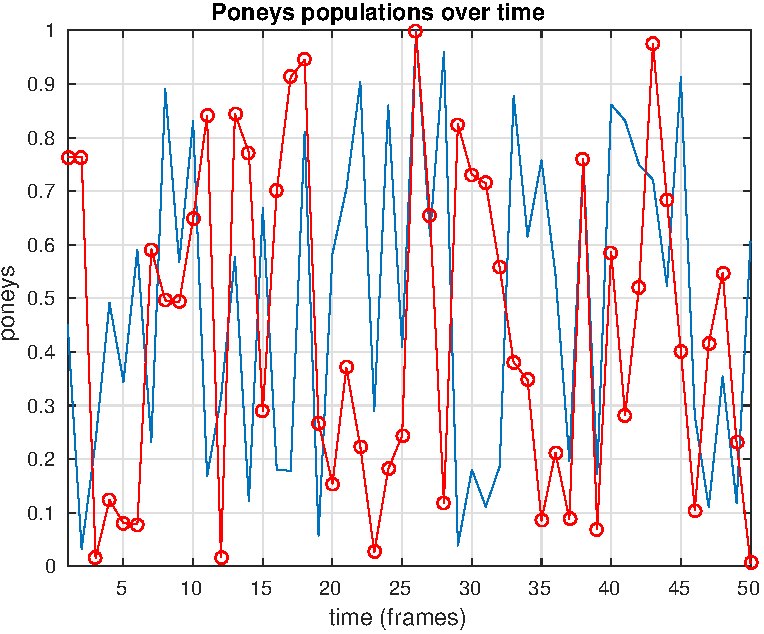
\includegraphics[width=0.5\textwidth]{basicplot.pdf}
  \caption{Basic plot}\label{fig:basic}
\end{figure}

You will now learn to plot vectors and arrays of random numbers.
Line and point data are plotted to screen with the \mcode{plot} command.

For this exercise, you will create a new function called \mcode{testPlot} in a file name \verb|testPlot.m|, as follows:
\begin{lstlisting}
function testPlot
  % exercise function
  R1 = rand(1, 100);  % a vector of 100 random variables
  R2 = rand(1, 100);  % another vector of 100 random variables

end
\end{lstlisting}

Open the doc page for the \mcode{plot} command.
Read quickly the \textbf{Description} and \textbf{Example} sections, to see the possibilities of this function.

You will now add some lines to \mcode{testPlot} to display \mcode{R1} and \mcode{R2} in a fancy way.
We will give you the steps with the functions you should use.
Remember, you can (and \emph{should}) look at the documentation of the functions we will mention.
After each step, run your function (typing \mcode{testPlot} in the command line) to see your progress.
\begin{enumerate}
  \item Open a new empty figure window with \mcode{figure} function (1 new line).
  \item Use the \mcode{plot} function to display \mcode{R1} with the default settings (1 new line).
  \item \mcode{plot} can take a \textbf{string} input defining the type of the line.
    Look for \emph{LineSpec} information in \mcode{plot} documentation and/or look at the provided examples.
  \item Change the call to \mcode{plot} to display \mcode{R1} with a red line.
  \item Change the call to \mcode{plot} to display \mcode{R1} with red circles and lines.
  \item Try to display \mcode{R2} on the same graph with a new \mcode{plot} call. (1 new line)\\
    By default, MATLAB blanks previous graph if you call \mcode{plot} twice on the same figure.
    To desactivate this behaviour, you need to use \mcode{hold on} and \mcode{hold off} before and after
    your second \mcode{plot} call.
    Here is a fictional example, adapt it to your case! (2 new lines)
\begin{lstlisting}
plot(x)  % first graph
hold on
plot(y)  % second graph
hold off
\end{lstlisting}
  \item Add a title to your graph, using \mcode{title} function. (1 new line)
  \item Add fictional axes names to your graph, using \mcode{xlabel} and \mcode{ylabel} functions. (2 new lines)
  \item Display a grid on your graph, using \mcode{grid} function. (1 new line)
  \item Limit the x-axis display to the first 50 points, using \mcode xlim function. (1 new line)
  \item Be proud of your first graph and save it as a .png file using \emph{File/Save As\dots} menu in the figure window.
\end{enumerate}

The final result should look like figure~\ref{fig:basic}.

\subsection{Advanced plotting: subplots, images and histogram}

\begin{figure}
  \centering
  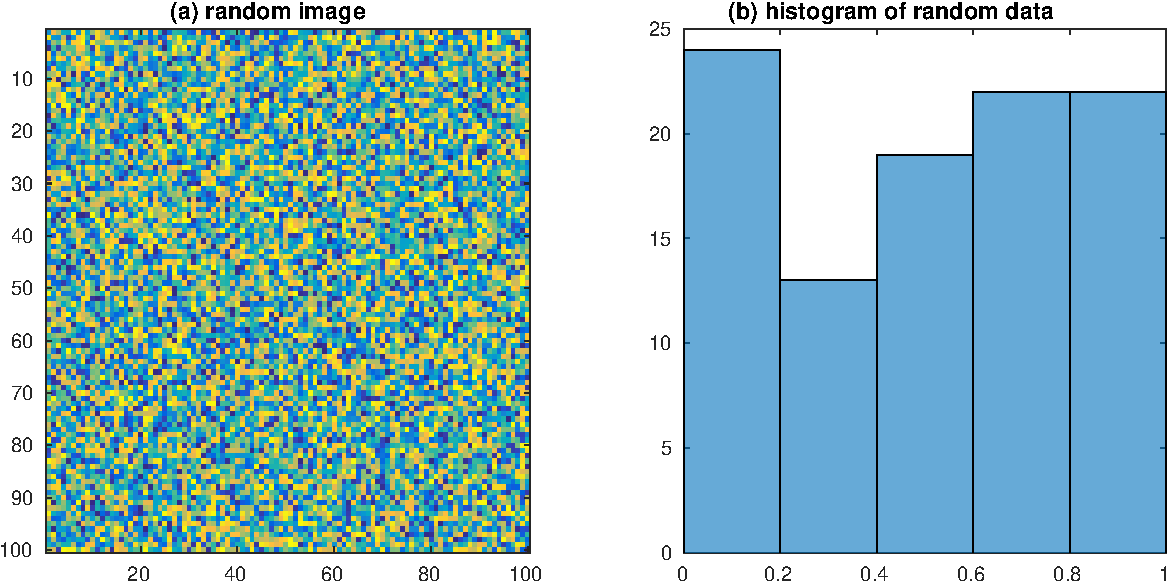
\includegraphics[width=0.7\textwidth]{advancedplot.pdf}
  \caption{Advanced plot}\label{fig:adv}
\end{figure}

You will give a try to more advanced graphical functions.
The aim is to plot side-by-side an image and an histogram of some random data.

First, create a new function \mcode{testSubplot} in a new file \verb|testSubplot.m|.
In this function, do the following steps that will lead you to success:
\begin{enumerate}
  \item create a 100-by-100 matrix of random data and store it in a variable \mcode{R1} (use \mcode{rand} function),
  \item create a vector of 100 random numbers and store it in a variable \mcode{R2},
  \item create a new empty figure window (use \mcode{figure} function),
  \item create a new sub-plot on the left of the figure (use \mcode{subplot} function, check its documentation, especially examples),
  \item display in this sub-plot \mcode{R1} as an image (use \mcode{imshow} or \mcode{imagesc}, check the difference between both),
  \item create a second sub-plot on the right of the figure (use \mcode{subplot} again),
  \item display the histogram of \mcode{R2} on this sub-plot (use \mcode{hist} or \mcode{histogram}),
  \item save your figure as a .png image.
\end{enumerate}

You should obtain something similar to figure~\ref{fig:adv}.


\section{Conditional expressions with \emph{if\dots else} statement}

\verb|Conditional expressions| are really important since they allow you to add logic to a function.
Indeed, an \textbf{if\dots else} statement is a way to make a part of your function executed or not depending on a condition.

Type the following in a new function \mcode{testIf}:
\begin{lstlisting}
function testIf
  a = 2;
  if a < 0
    disp('a is negative')
  end
  disp('this always runs')
end
\end{lstlisting}
and run it of course!

What happens if you change the value of \mcode{a} to \mcode{-3}?
What gets displayed?

This conditional expression starts with the \mcode{if} keyword, followed by the condition, then the code to be executed if the condition is true (i.e. equals 1), and finally the \mcode{end} keyword to delineate the expression.
In the previous example, depending on the value of \mcode{a}, the condition \mcode{a < 0} equals 0 or 1, and line 4 gets executed or not.

If the first condition is false, you can add another condition using \mcode{elseif} keyword, with its own code to execute if true.
Note that it is possible to chain several \mcode{elseif} conditions.
In case you want to execute something if all previous conditions were false, you can use an \mcode{else} keyword followed by the code to be executed.

Here is an example that make use of all these constructs.
Change the value of the variable \mcode{a} and see how the function behaves.
\begin{lstlisting}
function testIf
  a = 2;
  if a < 0
    disp('a is negative')
  elseif a >= 5
    disp('a is superior or equal to 5')
  elseif a == 1
    disp('a is equal to 1')
  else
    disp('a is 2, 3 or 4')
  disp('this always runs')
end
\end{lstlisting}


\section{Repeating operations with \emph{for} loop}

Sometimes you might want to repeat some actions a finite number of case.
A \emph{bad} way to do this is to copy/paste lines and change values in each line to fit your needs.
A \emph{good} way to achieve this repetition is to use a \textbf{for}-loop construct.

A \textbf{for}-loops is used when the number of repetitions is known in advance.
The following function gives you a typical example:
\begin{lstlisting}
function testForLoop
  % loop from 1 to 10
  for ii=1:10
    disp('Loop 1')
    disp(ii)  % display current value of ii
  end

  % loop from 1 to 100, with increment of 10
  for jj=1:10:100
    disp('Loop 2')
    disp(jj)  % display current value of jj
  end
end
\end{lstlisting}

How many lines are printed by MATLAB when you run this function?
Quite a lot compared to the number of lines written, isn't it?

The \textbf{for}-loop starts with the \mcode{for} keyword, followed by the increment expression (e.g. \mcode{ii=1:10}), then the code for each iteration and finally the \mcode{end} keyword to close the loop definition.
At each iteration, the loop variable (\mcode{ii} and \mcode{jj} in example loops) gets the next value from the vector defined on the right of the \mcode{=} (equal) symbol.

Complete the following function to make it multiply each element of the variable \mcode{R1} by 2:
\begin{lstlisting}
function multiplyLoop
  % exercise function

  R1 = rand(12);  % initialize R1 with random values
  disp(R1);       % display initial R1

  % HERE, YES RIGHT HERE, YOU SHOULD PUT A LOOP.

  disp(R1)        % display updated R1
end
\end{lstlisting}

In general, even if loops are great, you can do the same operations more efficiently using arrays indexing and functions.
Rewrite the previous function \mcode{multiplyLoop} without loop.


\section{(Bonus) More exercises}

The following exercises should be done in a separate function for each of them.

\begin{enumerate}

\item Use \mcode{rand}, \mcode{round}, and \mcode{*} to produce a vector of 5000 random integers having values between 0 and 20.
Use the \mcode{unique} command to confirm that you have values from 0 to 20 and no others.
Use the \mcode{hist} command to make a histogram of the distribution.
Plot the histogram with 21 bins, since you have that many unique numbers.
Does it look like a uniform distribution? Replace \mcode{round} with \mcode{ceil} and repeat.
Is it uniform now?

\item Using the random vector you generated in the previous exercise, apply the \mcode{find} command and the \mcode{length} command to count the number of times the number 10 occurred.
  Does this number match what the histogram showed?

\item Repeat the previous exercise (ignoring the histogram) and count how many times a number less than or equal to two occurred.
  Repeat again and count the number of times a number less than or equal to three occurred.
  Now write a \mcode{for} loop that performs this count for all numbers between 1 and 20 (which are the unique numbers in the vector).

\item Build a 9 by 10 array. Plot this in an array of 3 by 3 subplots.
  Each subplot contains data from one row of the matrix (hint: array indexing).
  Waveforms should be red lines with no symbols.
  Add a green circle at the maximum value of each plot (hint: help max).

\end{enumerate}

\section{Additional resources}

You want more?
Right, here are some nice online resources to complete and go beyond this tutorial:
\begin{itemize}
  \item the MIT MATLAB course,\footnote{%
    \url{http://ocw.mit.edu/courses/electrical-engineering-and-computer-science/6-094-introduction-to-matlab-january-iap-2010/}
  }
  \item tutorialspoint.com course,\footnote{%
    \url{http://www.tutorialspoint.com/matlab}
  }
  \item Software Carpentry tutorial.\footnote{%
    \url{http://swcarpentry.github.io/matlab-novice-inflammation/}
  }
\end{itemize}

The last website, Software Carpentry, is a golden mine for data analysis.
Check their lessons\footnote{\url{http://software-carpentry.org}} if you want to learn more about other tools and programming languages used to crunch data and extract the best of them.

Happy analysis!

\end{document}
